\newpage
\section{Introduction}
Kinematic simulation is an important tool for many problems. For example, it is used to study the degrees of freedom or range of motion for linkage systems, or to simulate motion for virtual reality training, video games, rapid digital prototyping, and robotics simulation \cite{SiggraphContact22}.
For structural systems, it allows one to study whether or not a system is stable. For example, understanding the kinematic properties of thick origami is important if it were to be used structurally. A kinematic simulation would show which forces would cause the origami to deform without resistance \cite{filipov2015toward}. 
For our project, we wanted to develop a kinematic simulation library for thick, rigid origami so we could become more familiar with kinematic simulation methods and develop performant software that others could use. To test our package, the kinematic folding motions for a cube folded from flat and Miura origami pattern were simulated. The objectives of this project aimed to incorporate the course themes and were defined as follows: 
\begin{itemize}
    \item The library shall be able to simulate the kinematics any convex rigid body that can be sufficiently described by its vertices.
    \item The library shall make use of performant linear algebra libraries.
    \item The library shall make use of Object-Oriented Design.
    \item The library shall make use of design patterns.
    \item The library shall use a CMake based build system.
    \item The library shall use C++ mainly and C if needed.
    \item The library shall incorporate testing.

\end{itemize}


\subsection{Kinematic Simulations}
The kinematics of an origami object can be simulated by first defining the origami's mesh based on predefined nodes, then imposing constraints on those nodes' degrees of freedom based on the defined mesh, and finally, solving for the mesh's kinematically admissible motion based on the constraints \cite{zhu2022review}. 
%
\begin{figure}[H]
    \centering
    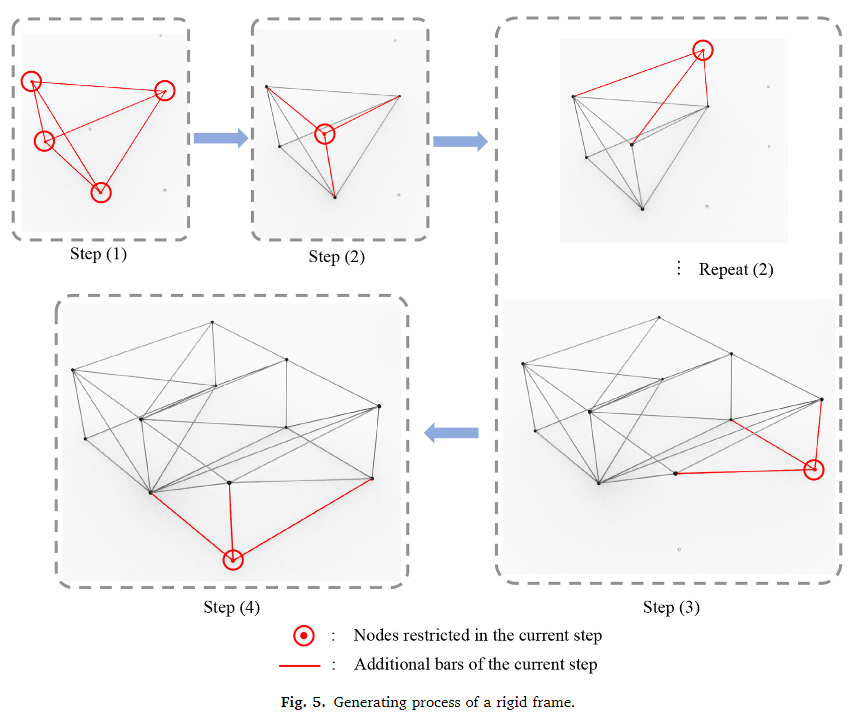
\includegraphics[width=0.6\columnwidth]{Graphics/mesh_gen.png}
    \caption{Procedure for generating a mesh given predefined nodes \cite{zhang2021folding}.}
    \label{fig:mesh_gen}
\end{figure}
%
To simulate the kinematics of an object, it first needed to be represented mathematically, which was done by creating a mesh of the object. There are many methods for creating meshes, but we used the one described in \cite{zhang2021folding} because it creates a mesh of edges and nodes that is automatically stable and minimally rigid.

This algorithm begins with a list of nodes that describe the important features of a convex hull, such as any corners. From here, four nodes are chosen randomly such that they create a tetrahedron, and links are defined between them. Then, another point is chosen randomly and connected to three existing points such that they all form another tetrahedron. Links are created between the three existing nodes and the new node. This process was repeated for all remaining nodes. Figure \ref{fig:mesh_gen} illustrates this. This process created the mesh for one rigid object, but to have objects that could develop complex motion, one or more objects needed to be connected. This was taken care of by grouping objects as bodies.

\subsubsection{Constraints}
Once all points were connected, a connectivity matrix could be formed, and from this, the constraints could be formed. 
The constraint equations of a kinematic system determine what motions are admissible. Constraint equations are determined by conditions such external physics, contact, friction, or geometry. For this library, we focused on purely geometrical constraints, where nodal locations of a rigid body must retain their originally specified distance from each other. If nodes $i$ and $j$ are connected by an edge, then their constraint equation would be
\begin{equation}\label{eq:edge}
    (u_i-u_j) \cdot (u_i-u_j) = l_{ij}^2,
\end{equation}
where $l_{ij}$ is the original distance between nodes $i$ and $j$, and $u_i$ is the coordinate of node $i$. Essentially, this constraint ensures the lengths of the edges remain constant throughout the folding motion.
Rigid bodies were connected along their nodes, where a node might belong to multiple edges. Each constraint defined by the edges was then linearized by taking its derivative with respect to time.
\begin{equation}\label{eq:con-linearized}
\frac{d}{dt}(u_i-u_j) \cdot (u_i-u_j) = \frac{d}{dt}l_{ij}^2.
\end{equation}
Since the body was rigid, its time derivative must be zero,
\begin{equation}\label{eq:con-rigid}
(u_i-u_j) \cdot (\dot u_i-\dot u_j) = 0,
\end{equation}
where Equation \ref{eq:con-rigid} can be decomposed into its cartesian components,
\begin{equation}\label{eq:con-components}
(x_i-x_j) (\dot x_i - \dot x_j)+(y_i-y_j) (\dot y_i - \dot y_j)+(z_i-z_j) (\dot z_i - \dot z_j) =0.
\end{equation}
This constraint was then defined for each pair of nodes connected by an edge, which yielded the system of equations,
\begin{equation}\label{eq:con-system}
C \dot d = 0,
\end{equation}
where $\dot d$ was a vector of velocities for each node's degrees of freedom,
$\dot d = [\dot x_0,\dot y_0,\dot z_0,\dots,\dot z_n]^T$.
Finally, some nodes needed to be constrained relative to the global coordinate system (i.e. boundary conditions). These were called \textit{fixities}. Fixities were implemented into the system of equations by requiring the specified degree of freedom's velocity to be zero and adding the appropriate equations to the constraint matrix.
\begin{equation}\label{eq:con-fixities}
\dot x_i = 0 
\end{equation}

\subsubsection{Admissible Motion}
The constraint matrix encodes all requirements for valid motion. Once the constraint matrix was defined, kinematically admissible velocities could be computed by solving Equation \ref{eq:con-system}. However, $C \in \mathbb{R}^{n \times k}$  where $n < k $, so this system of equations has many solutions. An easier way to find kinematically admissible velocities was to project a target velocity profile onto the null space of the constraint matrix.
\begin{equation}\label{eq:null-space}
\dot d = (I-C^{+}C)\dot d_0
\end{equation}
Where $C^+$ is the pseudo-inverse of $C$ and $\dot d_0$ is the target velocity.
In this way, the admissible velocity closest to the target velocity was chosen. Any numerical integration method may then be used to compute the displacements caused by these velocities. The simplest ODE solving scheme (but most likely to cause errors for long simulations) is the Euler method:
$$d_{i+1}=d_{i}+h\dot d_{i}$$

Where $h$ is the time step. Choosing a time step that is too large leads to larger distortion of the rigid bodies during simulation. Other methods that can be used are Heun's Method or any Runge-Kutta Method. These higher order iteration schemes would reduce the amount of error.


